\documentclass{article}

\usepackage{amsmath}
\usepackage{amssymb}
\usepackage{amsthm}
\usepackage{pgfplots}
\usepackage{tikz}\usetikzlibrary{decorations,arrows,arrows.meta,positioning}
\usepackage{booktabs}
\usepackage{xcolor}
\usepackage{float}
\usepackage{array}
\usepackage{tabu}
\usepackage{amsfonts}
\usepackage{bold-extra}
\usepackage{multirow}
\usepackage{mathrsfs}
\usepackage{url}
\usepackage{xspace}
\usepackage{hyperref}\hypersetup{colorlinks=true}
\usepackage[capitalise,noabbrev]{cleveref}
\usepackage{parskip}
\usepackage{listings}
\usepackage[a4paper]{geometry}

\begin{document}

\title{\textbf{Agora DRep Effect Specification}}
\author{
  Tomasz Maciosowski\\\href{mailto:tomasz@mlabs.city}{tomasz@mlabs.city} \and
  Gergely Szab\'o \\\href{mailto:gergely@mlabs.city}{gergely@mlabs.city}}
\date{}

\clearpage
\maketitle
\vskip 5mm
\begin{abstract}
  DAOs that have large treasuries of ADA tokens under their control cannot use that to directly participate in Cardano-level protocol governance introduced in the Chang hard fork.
  They would need to delegate their stake to a dRep and rely on them as a centralized party that should reflect the values of the whole organization.
  Instead, we propose to create a dRep onchain validator.
  DAOs should be able to delegate their treasuries to dRep validators that they directly control.
  Using Agora proposals, organization members will be able to decide how their DAO will vote instead.
\end{abstract}
\vskip 5mm
\section{Overview}

This document provides a specification of a set of Cardano validators that together provide Agora effect that
allows DAO members to use Agora voting system to decide how they want to act on Cardano-level governance proposal together as an organization.
Plutus V3 script can be registered as a Cardano DRep and we will use that to create a Plutus DRep that will allow voting on Cardano proposals only after the organization has passed a successful ``internal'' vote on that decision using their Agora instance.
First iteration of the DRep Effect will be limited in governance actions it is allowed to do only to voting, i.e. it will not be able to create Cardano governance proposals.
The implementation of this specification will be done in Plutarch and available on GitHub.

\subsection{V2 / V3 Interactions Limitations}

The Cardano ledger imposes limitations on what transaction can do depending on which versions of Plutus scripts are being executed in the same transaction.
The limitation that is relevant for us is that transactions that execute V2 Plutus scripts cannot also contain Cardano governance voting actions (see Table \ref{tab:compatibility}).

\begin{table}[H]
  \centering
  \begin{tabular}{l|l|l|l}
    Feature              & Plutus V2 & Plutus V3 & Plutus V2 + V3 \\
    \hline
    Plutus V1 Primitives & Yes       & Yes       & Yes            \\
    Governance Voting    & No        & Yes       & No             \\
  \end{tabular}
  \caption{\label{tab:compatibility}Part of Cardano Script Compatibility Chart}
\end{table}

The Plutus V2 script in question is the minting policy of the Governance Authority Tokens (GAT) of already deployed Agora instances.
It is important for organizations to continue using their current Agora instances so rather then requiring them to re-deploy Agora using Plutus V3 we will provide a GAT migration mechanism - a proxy validator that will convert GATs from V2 to V3 on demand.
More over the migration mechanism is separate from the voting effect thus may be used for other effects that need access to transaction features that were introduced after Plutus V2.

\section{Validators}

\subsection{Proxy Spending Validator}

Plutus V2 Agora instances can use this validator to use effects that are implemented in newer Plutus versions.
To do so instead of specifying actual effect in the proposal datum the user can specify this validator instead and specify the final V3 GAT destination using datum of the Proxy Spending Validator.
As a security measure the datum allows only for script destinations to make sure that GAT never reaches a public key address as it may compromise the whole Agora system.
Proxy Spending Validator is parametrized by the real Agora Governance Authority Token symbol and allows for spending only if it's UTxO contains that GAT and the transaction burns it.

Note that the actual minting will be done by Proxy Minting Validator.
While they are described as two separate validators actually they will be the same onchain script that acts differently depending on the purpose it is spent with.
That approach avoids circular script parametrization as minting part needs to know the address of the spending part and spening part needs to know the currency symbol of the minting part, if they are implemented in the same script that then the script hash is the same and it is passed as a runtime parameter from Cardano node.

For the sake of simplicity and correctness the implementation is limited to migrating only one GAT per transaction.
In practice such limitation is irrelevant as most Agora proposals have only one effect in the outcome map and proposals are rare enough that the cost of submitting multiple transactions is irrelevant.

Note that this validator is in fact an Agora effect thus the spending conditions must follow the restrictions for Agora effects such as not doing anything that is irrelevant to the GAT migration process as that may accidently allow to trigger other action that is gated behind burning V2 GAT.

\subsubsection*{Data Types}

\begin{lstlisting}[language=Haskell]
data Datum = Datum
  { receiverScript :: ScriptHash
  , datumHash :: DatumHash
  }
\end{lstlisting}

\subsubsection*{Spending Conditions}

\begin{itemize}
  \item Transaction burns one GAT (symbol is known from script parameter)
  \item Spent UTxO contains GAT
  \item Transaction creates a UTxO at address of \verb|receiverScript| with empty staking part and reference datum with hash equal to \verb|datumHash|.
  \item Transaction does not mint or burn any tokens other than V2 and V3 GATs.
  \item Transaction does not include any certificates.
  \item Transaction does not include script inputs other than own input.
\end{itemize}

\subsection{Proxy Minting Validator}

Minting validator is tightly coupled to the spending validator and some checks are offloaded there. This validator succeeds when the transaction spends from the spending validator address (that already ensures proper handling of V2 GAT) and that it mints exactly one V3 GAT with empty token name.

\subsubsection*{Spending Conditions}

\begin{itemize}
  \item Transaction contains an input from Proxy Spending Validator. The address is known as Minting and Spending validators share the same hash.
\end{itemize}

\subsection{Spending Effect Validator}

Because onchain voting action is gated behind burning pGAT the effect implementation has to be split into spending and voting validators. Spending validator simply allows only for burning the pGAT as long as the transaction.

\subsubsection*{Spending Conditions}

\begin{itemize}
  \item Transaction contains a vote with own drep hash
\end{itemize}

Rest  of the checks if performed by the Voting Effect validator.

\subsubsection*{Interaction diagrams}

\begin{figure}[H]
  \begin{center}
    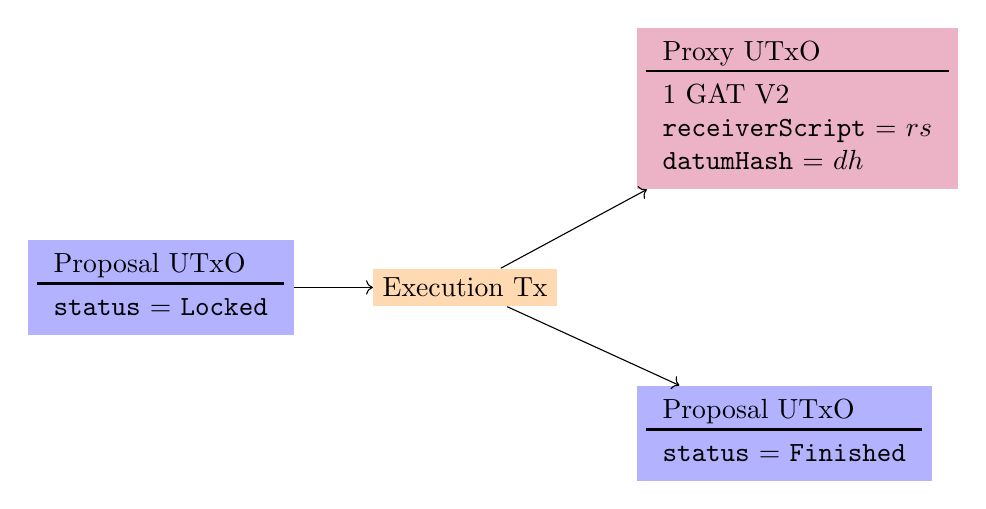
\begin{tikzpicture}
      \node[shape=rectangle,fill=orange!30](tx) {Execution Tx};
      \node[shape=rectangle,fill=blue!30,left=of tx](p1) {
        \begin{tabular}{l}
          Proposal UTxO \\ \toprule
          \verb|status| = \verb|Locked|
        \end{tabular}
      };
      \node[shape=rectangle,fill=blue!30,below right=of tx](p2){
        \begin{tabular}{l}
          Proposal UTxO \\ \toprule
          \verb|status| = \verb|Finished|
        \end{tabular}
      };
      \node[shape=rectangle,fill=purple!30,above right=of tx](gat){
        \begin{tabular}{l}
          Proxy UTxO                   \\ \toprule
          1 GAT V2                     \\
          \verb|receiverScript| = $rs$ \\
          \verb|datumHash| = $dh$
        \end{tabular}
      };
      \draw[->] (p1) -- (tx);
      \draw[->] (tx) -- (p2);
      \draw[->] (tx) -- (gat);
    \end{tikzpicture}
  \end{center}
  \caption[]{Minting V2 GAT}
\end{figure}

\begin{figure}[H]
  \begin{center}
    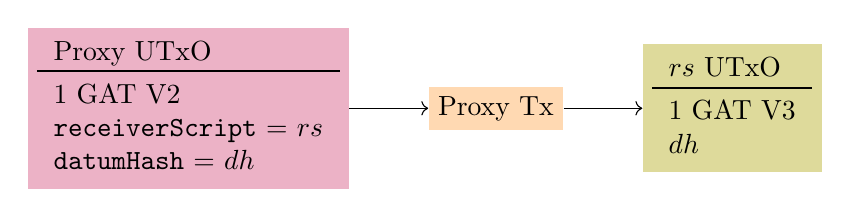
\begin{tikzpicture}
      \node[shape=rectangle,fill=orange!30](tx) {Proxy Tx};
      \node[shape=rectangle,fill=purple!30,left=of tx](gat1) {
        \begin{tabular}{l}
          Proxy UTxO                   \\ \toprule
          1 GAT V2                     \\
          \verb|receiverScript| = $rs$ \\
          \verb|datumHash| = $dh$
        \end{tabular}
      };
      \node[shape=rectangle,fill=olive!30,right=of tx](gat2){
        \begin{tabular}{l}
          $rs$ UTxO \\ \toprule
          1 GAT V3  \\
          $dh$
        \end{tabular}
      };
      \draw[->] (gat1) -- (tx);
      \draw[->] (tx) -- (gat2);
    \end{tikzpicture}
  \end{center}
  \caption[]{GAT Upgrade to V3}
\end{figure}

\subsection{Voting Effect Validator}

The Voting Effect validator will utilise the above established Proxy Minting Validator, minting a Proxy Governance Authority Token (pGAT).
By spending the pGAT, we essentially get the same guarantees as with GAT, but we can use Plutus V3, which introduces the functionalities to work with native Cardano governance.
Similarly to the Proxy Validator, the script serves multiple purposes, to avoid the circular dependency problem (see explanation in 2.1 Proxy Spending Validator).

In order to vote on a Cardano Governance Action using this effect the following preconditions must be met:
\begin{itemize}
  \item The Voting Effect validator must be registered as a DRep
  \item staking verification key of the DAO should be delegated to the above DRep
  \item Governance action with well known id must be already submitted on-chain
\end{itemize}

The effect transaction will burn exactly one pGAT, and at the same time place a vote to the governance action defined in the datum.

\subsubsection*{DRep registration}

Registering the Voting Effect validator is a one time action, that has to be done after deployment of the protocol.
The validator script will allow DRep registration unconditionally, but DRep update will be prohibited.

\subsubsection*{Data Types}

\begin{lstlisting}[language=Haskell]
data Datum = Datum
  { governanceActionId :: GovernanceActionId
  , vote :: Vote
  }
\end{lstlisting}

\subsubsection*{Spending Conditions}

\begin{itemize}
  \item \verb|ScriptPurpose| is either \verb|Certifying|, \verb|Voting|, or \verb|Spending|
        \begin{itemize}
          \item if \verb|Spending|
                \begin {itemize}

          \item \verb|ScriptContext| contains exactly 1 script input
          \item \verb|ScriptContext| contains exactly 1 vote where the \verb|Voter| is the DRep credential of the Voting Script (script hash is common with the spending script)
        \end{itemize}
  \item if \verb|Certifying|
        \begin{itemize}
          \item \verb|ScriptContext| contains exactly 1 transaction DRep registration certificate
          \item \verb|ScriptContext| does not contain a vote
          \item \verb|ScriptContext| does not contain proposal procedures
          \item \verb|ScriptContext| does not contain treasury donations
        \end{itemize}
  \item if \verb|Voting|
        \begin{itemize}
          \item above input has \verb|Voting Effect datum| as a hashed datum
          \item \verb|ScriptContext| contains exactly 1 vote, where the \verb|GovernanceId| and \verb|Vote| match the ones in the \verb|Voting Effect's datum|
          \item \verb|ScriptContext| does not contain a certificate
          \item \verb|ScriptContext| does not contain proposal procedures
          \item \verb|ScriptContext| does not contain treasury donations
        \end{itemize}


\end{itemize}
\end{itemize}

\subsubsection*{Interaction Diagrams}

\begin{figure}[H]
  \begin{center}
    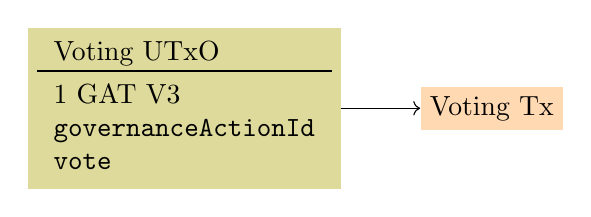
\begin{tikzpicture}
      \node[shape=rectangle,fill=orange!30](tx) {Voting Tx};
      \node[shape=rectangle,fill=olive!30,left=of tx](gat1){
        \begin{tabular}{l}
          Voting UTxO               \\ \toprule
          1 GAT V3                  \\
          \verb|governanceActionId| \\
          \verb|vote|
        \end{tabular}
      };
      \draw[->] (gat1) -- (tx);
    \end{tikzpicture}
  \end{center}
  \caption[]{Voting}
\end{figure}

\begin{figure}[H]
  \begin{center}
    \begin{tikzpicture}
      \node[shape=rectangle,fill=orange!30](tx1) {Execution Tx};
      \node[shape=rectangle,fill=blue!30,above=of tx](p1) {
        \begin{tabular}{l}
          Proposal UTxO \\ \toprule
          \verb|status| = \verb|Locked|
        \end{tabular}
      };
      \node[shape=rectangle,fill=blue!30,below left=of tx](p2){
        \begin{tabular}{l}
          Proposal UTxO \\ \toprule
          \verb|status| = \verb|Finished|
        \end{tabular}
      };
      \node[shape=rectangle,fill=purple!30,below right=of tx](gat1){
        \begin{tabular}{l}
          Proxy UTxO                     \\ \toprule
          1 GAT V2                       \\
          \verb|receiverScript| = Voting \\
          \verb|datumHash| = $hash(\verb|governanceActionId, vote|)$
        \end{tabular}
      };
      \draw[->] (p1) -- (tx1);
      \draw[->] (tx1) -- (p2);
      \draw[->] (tx1) -- (gat1);

      \node[shape=rectangle,fill=orange!30,below=of gat1](tx2) {Proxy Tx};
      \node[shape=rectangle,fill=olive!30,below=of tx2](gat2){
        \begin{tabular}{l}
          Voting UTxO               \\ \toprule
          1 GAT V3                  \\
          \verb|governanceActionId| \\
          \verb|vote|
        \end{tabular}
      };
      \draw[->] (gat1) -- (tx2);
      \draw[->] (tx2) -- (gat2);

      \node[shape=rectangle,fill=orange!30,below=of gat2](tx3) {Voting Tx};
      \draw[->] (gat2) -- (tx3);
    \end{tikzpicture}
  \end{center}
  \caption[]{Full Workflow}
\end{figure}

\section{Data Encoding}

Datums and redeemers defined in this specification have to be data-encoded using the following rules in order to achieve the optimal encoding:

\begin{itemize}
  \item Enums (SoPs where all constructors have no fields) have to be encoded as an integer starting from $0$ following the constructor order from the specification.
  \item Records (SoPs with only one constructor with at least one field) have to be encoded as a list of data encoded fields rather than wrapped with \verb|Constr 0|.
  \item Everything else has to be encoded using \verb|Constr| with index starting from $0$ following the constructor from the specification and field list in order of the declaration.
\end{itemize}

Note that we do not ``mix'' the encodings i.e. even if one of the constructors of the generic SoP has no fields it still has to be encoded using \verb|Constr| rather than as an integer.
Types that are not defined in this document are standard Plutus types with encoding already specified and the encoding rules do not apply to them.

When the specification does not describe datum or redeemer it is assumed to be never accessed thus plutus data passed to the script is irrelevant and the offchain implementation is free to pass anything and the validator has to succeed anyway.
Usually the offchain transaction building code will pass unit type encoded as \verb|Constr 0 []| or \verb|0| however it is not strictly required to do so.

\subsection{Plutarch Details}

Note that the following encodings can be achieved automatically using Plutarch's derivation strategies, namely:

\begin{itemize}
  \item Enum encoding can be derived with \verb|DeriveAsTag| for both \verb|PlutusType| and \verb|PLiftable|
  \item Record with \verb|DeriveAsDataRec| for \verb|PlutusType| and \allowbreak \verb|DeriveDataPLiftable| for \verb|PLiftable|
  \item Generic SoP encoding can be derived with \verb|DeriveAsDataStruct| for \verb|PlutusType| and \verb|DeriveDataPLiftable| for \verb|PLiftable|
\end{itemize}

\section{Estimate}

\begin{itemize}
  \item Milestone 1 (Spec): 199 hours
        \begin{itemize}
          \item 75 h - Research spending, minting, and voting conditions
          \item 62 h - Draft specifications for each validator
          \item 62 h - Create a detailed LaTeX document for the conditions
        \end{itemize}

  \item Milestone 2 (Proxy Implementation): 182 hours
        \begin{itemize}
          \item 62 h - Develop the proxy spending validator using Plutarch
          \item 62 h - Implement the V3 minting policy
          \item 58 h - Set up a GitHub repository for the project
        \end{itemize}

  \item Milestone 3 (Spending/Voting Implementation): 182 hours
        \begin{itemize}
          \item 68 h - Create a comprehensive test suite for the proxy validator
          \item 54 h - Conduct code reviews
          \item 46 h - Validate the implementation using test cases
          \item 14 h - Document results in a test report
        \end{itemize}

  \item Milestone 4 (Off-chain \& Frontend Integration): 234 hours
        \begin{itemize}
          \item 89 h - Develop the spending effect validators in Plutarch
          \item 74 h - Write test cases for the spending validators
          \item 57 h - Review and validate the code with tests
          \item 14 h - Upload the code to GitHub
        \end{itemize}

  \item Milestone 5 (Documentation): 234 hours
        \begin{itemize}
          \item 90 h - Develop the voting effect validators in Plutarch
          \item 58 h - Write and execute test cases for voting validators
          \item 58 h - Conduct final code reviews and validation
          \item 28 h - Ensure documentation and upload the code to GitHub
        \end{itemize}

  \item Milestone Final (End-to-End Testing): 300 hours
        \begin{itemize}
          \item 101 h - Develop off-chain components for clarity.vote integration
          \item 71 h - Implement frontend interface for proposals and voting
          \item 71 h - Create API documentation and tutorial guides
          \item 57 h - Test on Testnet and prepare a closeout report with a demo video
        \end{itemize}
\end{itemize}
Total: 1331 h

\end{document}
